\icode{E-MCH-SI-L2-261026-002}
在同一平台上的\(O\)点抛出的2个物体,做平抛运动的轨迹如图所示，则2个物体做平抛运动的初速度\(v_a\)、\(v_b\)的关系及落地时间\(t_a\)、\(t_b\)的关系分别是\paren[]

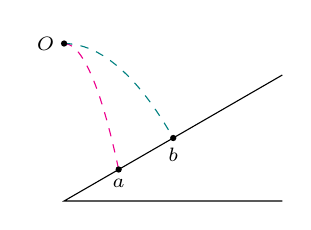
\begin{tikzpicture}[font=\scriptsize]
	\draw[dashed,magenta] (0,2)coordinate(O) parabola bend (0,2) (30:.8)coordinate(a);
	\draw[dashed,teal] (0,2) parabola bend(0,2) (30:1.6)coordinate(b);
	\draw ({3.2*cos(30)},0)--(0,0)--(30:3.2);
	\foreach \c/\t in {O/left,a/below,b/below}
		\fill (\c)node[\t]{ \(\c\)} circle(.04);
\end{tikzpicture}
\begin{choices}
	\item \(v_a > v_b\)\quad \(t_a > t_b\)
	\item \(v_a > v_b\)\quad \(t_a < t_b\)
	\item \(v_a < v_b\)\quad \(t_a > t_b\)
	\item \(v_a < v_b\)\quad \(t_a < t_b\)
\end{choices}
\begin{answer}
	C\qquad 提示：
\end{answer}